\begin{surferPage}[Quintic (15 Cusps)]{Una quintica con 15 cuspidi}
  Questa superficie di grado $5$ (quintica) ha $15$ singolarit\`a di tipo $A_2$
    (dette cuspidi); questa quintica insieme a una serie di superfici correlate \`e presa da un articolo del
  	 2005 di Oliver Labs.
    Cinque delle cuspidi hanno aspetto differente dalle altre dieci.
    In effetti, queste cinque sono singolarit\`a di tipo $A_2^{++}$, le altre di tipo $A_2^{+-}$ (vedi la galleria
    delle singolarit\`a semplici per maggior informazione):

     \vspace*{-0.3em}
    \begin{center}
      \begin{tabular}{c@{\qquad}c}
        \includegraphics[height=1.2cm]{./../../common/images/dessins_quint_15a2}
        &
        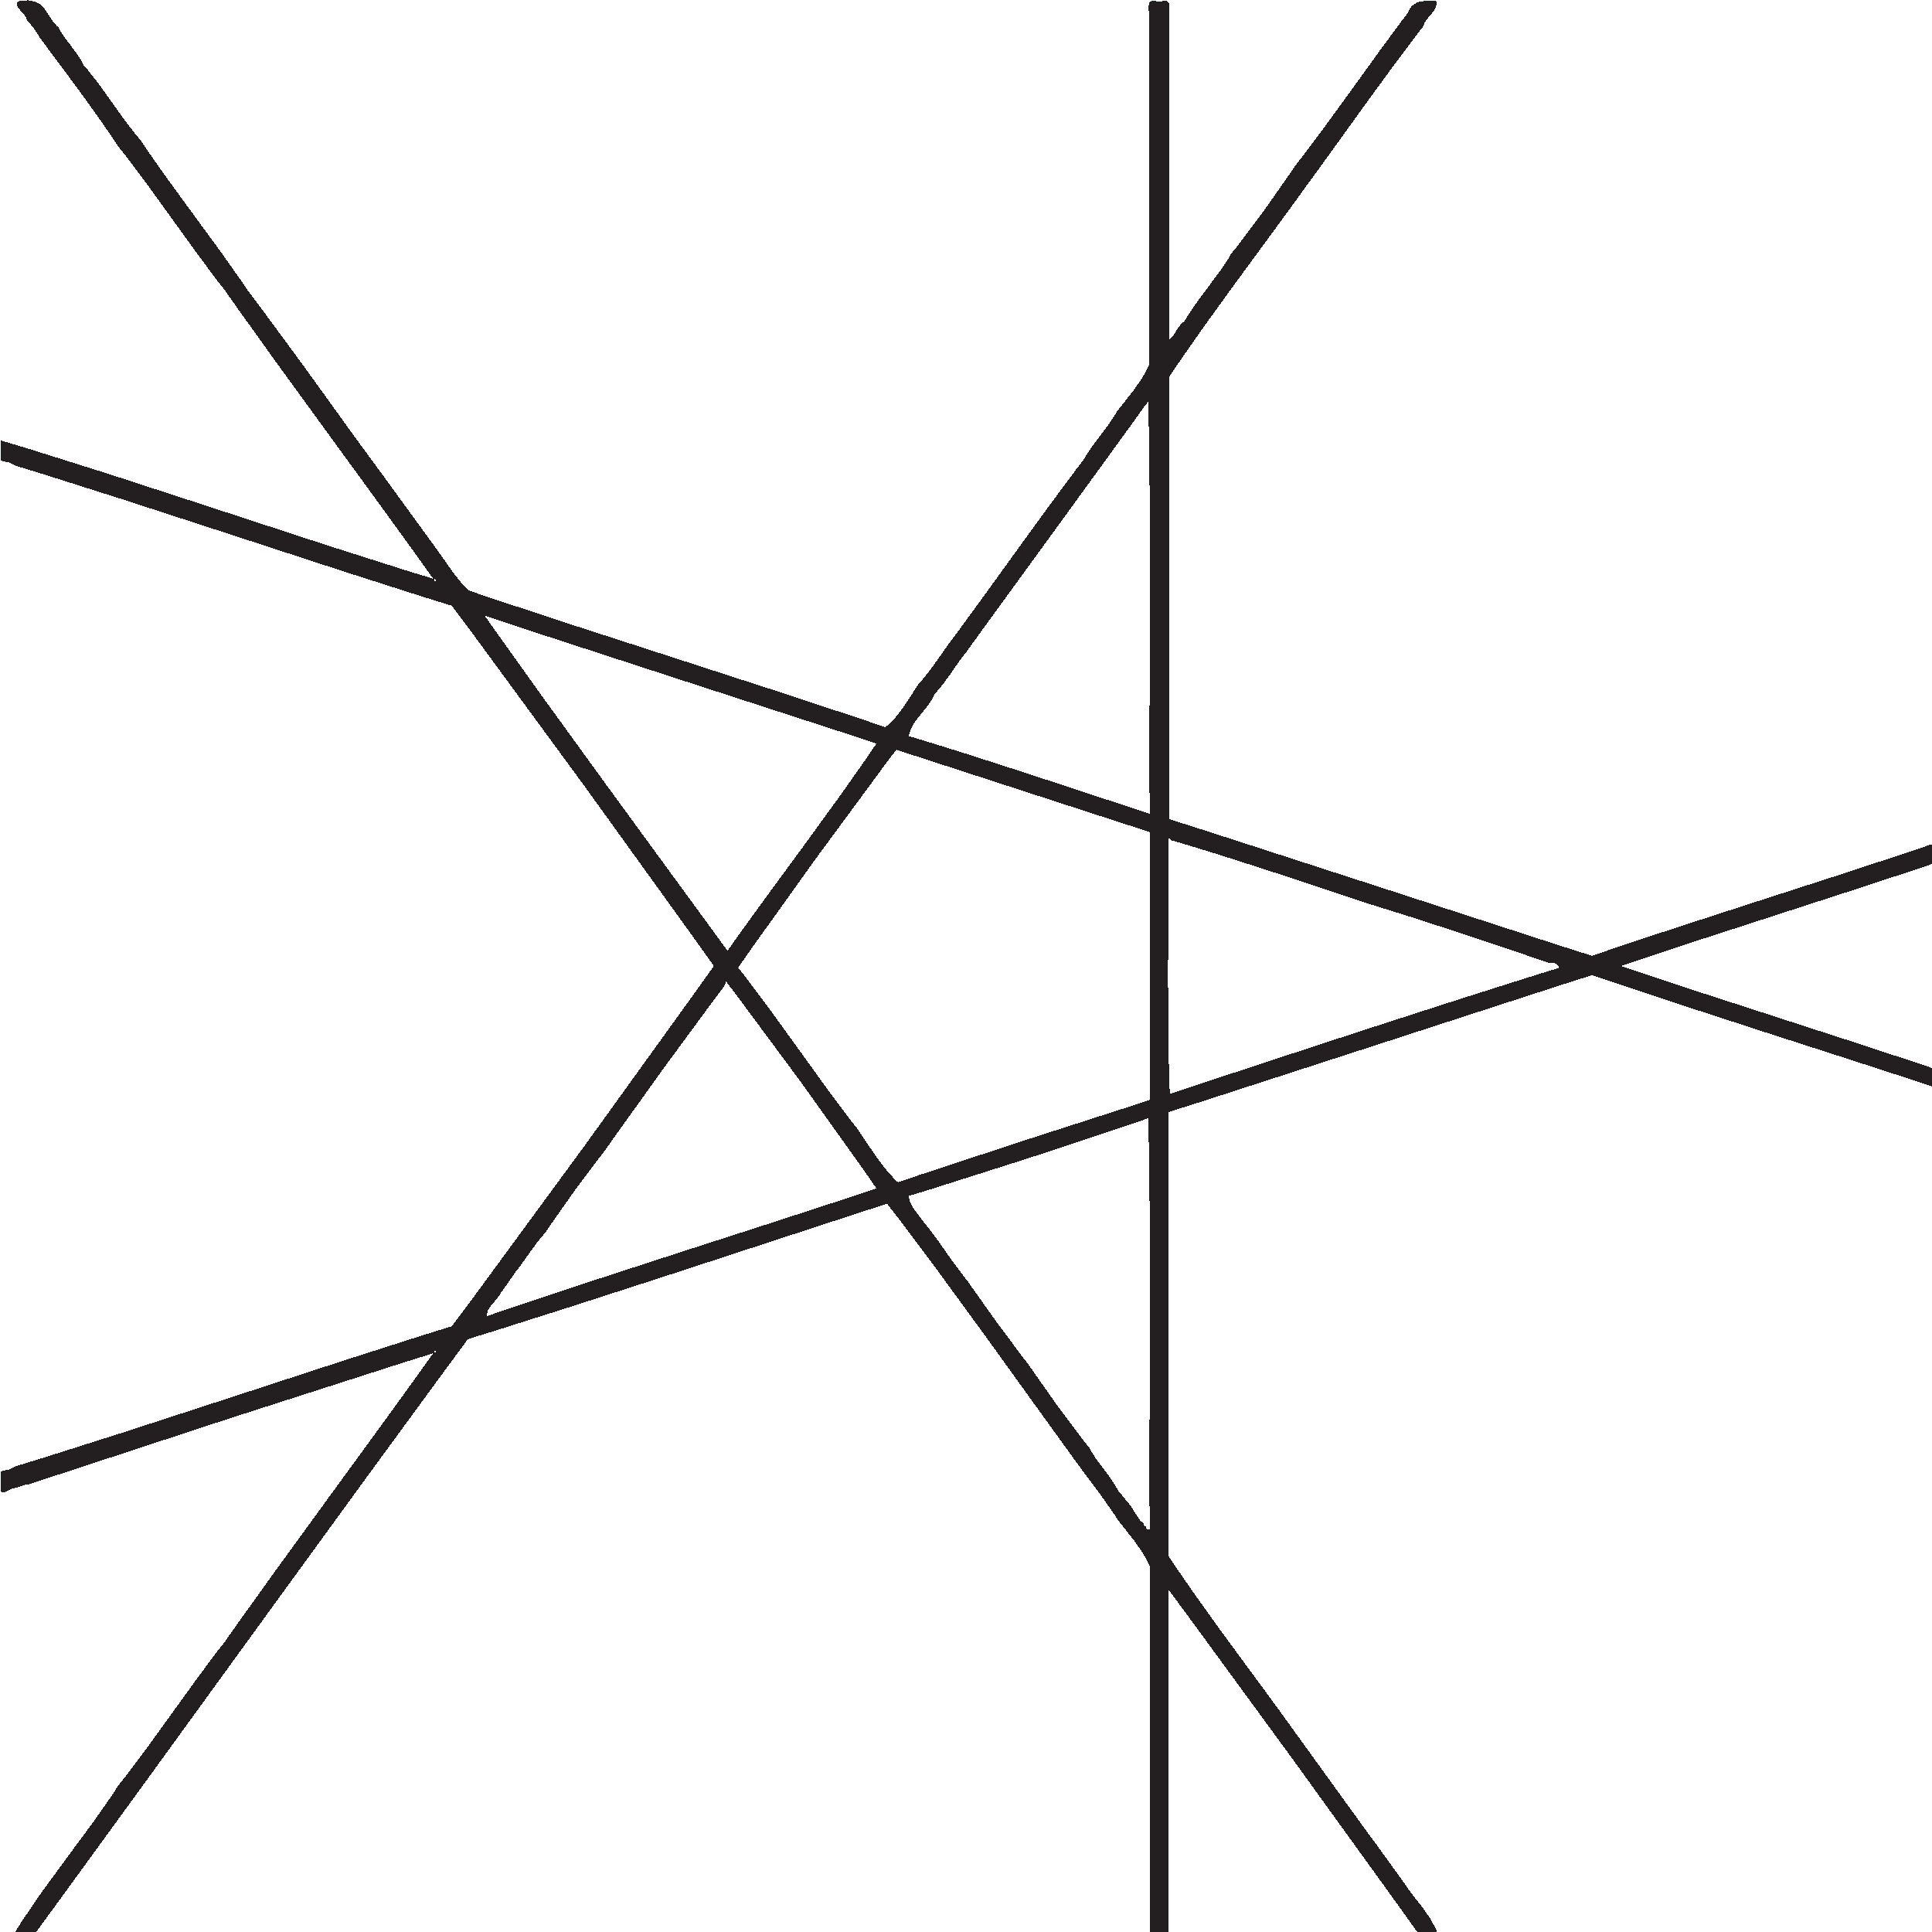
\includegraphics[height=1.2cm]{./../../common/images/rp5.pdf}
      \end{tabular}
    \end{center}
    \vspace*{-0.3em}    
    
    Questa superficie ha equazione della forma 
    $S_5(x,y) + t(z)=0,$
    dove $S_5(x,y)$ \`e un pentagono regolare (figura a destra) e $t(z)$ \`e una variazione dei polinomi di Tchebychev che abbiamo gi\`a menzionato diverse volte.

     Un'altra quintica (a sinistra) con $15$ cuspidi fu costruita da
    Wolf Barth; \`e collegata alla cubica di Clebsch (a destra) come si vede dalla figura al centro:

    \vspace*{-0.3em}
    \begin{center}
      \begin{tabular}{c@{\quad}c@{\quad}c}
        \includegraphics[height=1.2cm]{./../../common/images/barthquintic_green}
        &
        \includegraphics[height=1.2cm]{./../../common/images/barthquintic_clebschcubic}
        &
        \includegraphics[height=1.2cm]{./../../common/images/clebschcubic_pink}
      \end{tabular}
    \end{center}
    \vspace*{-0.3em}
\end{surferPage}
